\documentclass[addpoints,11pt]{exam}
\date{\today}
\usepackage{preamble}
%\printanswers %auskommentieren, um keine Loesungen zu sehen

    %Voreinstellungen zur Klassenarbeit 
\newcommand{\lehrname}{Erne}        %Name der unterrichtenden Lehrkraft
\newcommand{\ufach}{Mathematik}     %Fach
\newcommand{\lstniveau}{G-Kurs}	    %Leistungsniveau
\newcommand{\kanr}{1}               %Klassenarbeit-Nr
\newcommand{\kathema}{Lineare  und quadratische \linebreak Funktionen}%Thema, ggf. linebreak setzen
\newcommand{\zglhilf}{Taschenrechner}%Zugelassene Hilfsmittel
\newcommand{\bearbzeit}{60 Minuten}%Bearbeitungszeit

\runningheader{\ifcontinuation{Fortsetzung Aufgabe \ContinuedQuestion\ \ldots}{}}{Seite \thepage\ von \numpages}{\oddeven{}{\framebox(160,30){$\;$ Name: \hfill}}}
%\lhead{\ifcontinuation{Question \ContinuedQuestion\ continues\ldots}{}}
\begin{document}

\runningheadrule
\runningfootrule
\runningfooter{}{}{\ifincomplete{Aufgabe \IncompleteQuestion\ wird auf der nächsten Seite fortgesetzt}{}}

\firstpageheadrule

%\thispagestyle{headandfoot}
\newgeometry{left=1.5cm,
        right=1.5cm,
        top=4cm,
        bottom=1cm}
\coverheader
	{Lehrkraft: \lehrname\linebreak
		Fach: \ufach \linebreak
		\lstniveau}
	{\medskip\Large{\textbf{Klassenarbeit Nr. \kanr}} \linebreak
		\normalsize{\kathema}}
	{{\fontsize{12}{16}{\selectfont Name:\enspace\makebox[4cm]{\hrulefill}\linebreak Klasse:\enspace\makebox[4cm]{\hrulefill}\linebreak Datum:\enspace\makebox[4cm]{\hrulefill}}}}
\begin{coverpages}
%############################# DECKBLATT ################
\vspace*{-0.7cm}\hrule \vspace*{0.5cm}
\begin{large}
\textbf{Bearbeitungshinweise}
\end{large}
\begin{itemize}
\item Das Deckblatt darf erst auf Anweisung der Lehrkraft umgeblättert werden.
\item Tragt rechts oben euren Namen ein.
\item Die Bearbeitungszeit beträgt \bearbzeit .
\item Lest die Aufgaben in Ruhe und ganz genau durch.
\item Lösungswege und Rechnungen müssen nachvollziehbar sein.
\item Achtet auf gute Lesbarkeit, Rechtschreibung und Zeichensetzung.
\item Antwortsatz nicht vergessen!
\item Zugelassene Hilfsmittel: \zglhilf
\end{itemize}
\vspace*{0.3cm}
\begin{center}
\begin{huge}
Viel Erfolg!
\end{huge}
\linebreak
\includegraphics[scale=0.2]{smiley}
\linebreak
\hdashrule[0.1ex]{18.5cm}{0.5mm}{3mm 3pt} 
\end{center}
\begin{center}
\cellwidth{2.2em}
%TO DO: Anzahl der Zeilen von Anz. der Aufgaben abh.
\newcommand{\bwrtzeilen}{1}
%\multirowgradetable{\bwrtzeilen}[questions]
\INTEGERDIVISION{\totalquestions}{10}{\sola}{\solb}
\ADD{\sola}{1}{\numrows}
\multirowgradetable{%
  \numrows
}[questions]

\vspace*{0.7cm}
Diese Klassenarbeit besteht aus \numquestions\ Aufgaben. Insgesamt waren \numpoints\ Bewertungseinheiten (BE) zu erreichen. \smallskip

Du hast \underline{\hspace*{1.5cm}} BE erreicht. Das sind \underline{\hspace*{1.5cm}} Prozent. \medskip


\framebox(350,50){\textbf{Notenpunkte:} \underline{\hspace*{2cm}} \hspace*{1cm} \textbf{Note:} \underline{\hspace*{2cm}}}
\end{center}
\end{coverpages}
\restoregeometry
\newpage

\extraheadheight{0.7cm}
\extrafootheight{-1.5cm}
\firstpageheader{}{Seite \thepage\ von \numpages}{}
\begin{questions}

\question
Herr Meier verdient in zwei Stunden 34\euro.
\begin{parts}
\part[2] Fülle die Tabelle richtig aus \droppoints
\begin{table}[h!]
\centering
\begin{tabular}{|c|c|}
\hline
\rowcolor{Gray}
Anzahl der Stunden (x) & Verdienst in \euro \, (y) \\ \hline
1                      &           \\ \hline
2                      & 34        \\ \hline
4                      &           \\ \hline
6                      &           \\ \hline
7                      &           \\ \hline
\end{tabular}
\end{table}
\part[2] Kreuze an, mithilfe welcher Funktionsgleichung der Verdienst berechnet werden kann. \droppoints

\begin{oneparcheckboxes}
\choice $y=2x$
\choice $y=34x$
\choice $y=17x$
\choice $y=12x+2$
\choice $y=34x+2$
\end{oneparcheckboxes}
\end{parts}

\droptotalpoints

\question[3]
Berechne die fehlenden Werte in den Tabellen mithilfe der angegebenen Funktionsgleichungen.
$y = 2x+5$
%tables: https://tex.stackexchange.com/questions/7208/how-to-vertically-center-the-text-of-the-cells/611601#611601
\begin{table}[h!]
\renewcommand{\arraystretch}{1.2}
\hspace{1.5cm}\begin{tabular}{|G{1cm}|M{2cm}|M{2cm}|M{2cm}|M{2cm}|M{2cm}|M{2cm}|N}
\hline
x & -3 & -2 & -1 & 0 & 1 & 2 &\\ \hline
y & & & & & & &\\ \hline
\end{tabular}
\end{table}

\droptotalpoints

\question[2]
Gegeben ist die Funktion $f(x)=3x+4$. Die unten angegebenen Punkte liegen alle auf dem Graphen der Funktion $f$. Berechne die fehlende $y$-Koordinate der Punkte. 

$P_1(2|\loeslin) \qquad P_3(-1,5|\loeslin) $

\droptotalpoints

\question[3]

Gegeben sind die beiden Funktionsgleichungen $f_1(x)=2x+3$ und $f_2(x)=3x-4$. Trage die Punkte, die auf dem Graphen von $f_1$ liegen in die linke Spalte und die Punkte, die auf dem Graphen von $f_2$ liegen, in die rechte Spalte ein.
\begin{table}[h!]
\centering
\begin{tabular}{|M{3.2cm}|M{3.2cm}|}
\hline
\rowcolor{Gray}
$f_1$ & $f_2$ \\ \hline
                      &           \\ \hline
                      &           \\ \hline
                      &           \\ \hline
\end{tabular}
\end{table}
\begin{align*}
P_1&(4|11)  &  P_2&(2|2)    &  P_3&(5|11) &  P_4&(-3|-13) \\
\end{align*}
\droptotalpoints

\question[4]
Ordne den Funktionsgleichungen die richtigen Funktionsgraphen zu. 

\scalebox{0.8}{
\pgfplotsset{compat=1.18}
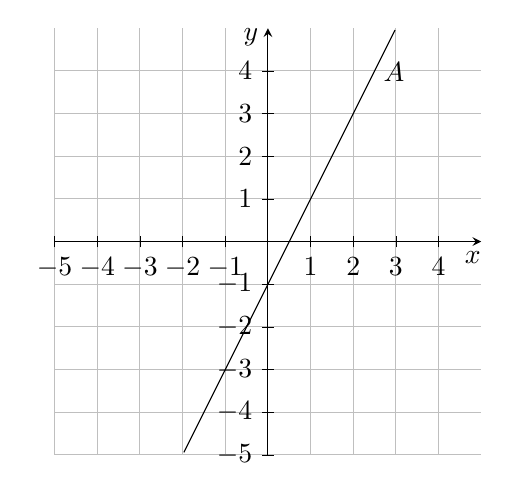
\begin{tikzpicture}[domain=-5:5,smooth]
  \begin{axis}[
      width=7cm,height=7cm,
      axis lines=middle,
      domain=-5:5,
      smooth,
      no markers,
      grid,
      xmin=-5,xmax=5,
      tick style=black,
      xtick={-5,-4,...,4},
      xlabel=$x$,
      xlabel style={below, anchor=north east,inner xsep=0pt},
      restrict y to domain=-5:5,
      ymin=-5,ymax=5,
      ytick={-5,-4,...,4},ylabel=$y$,
      ylabel style={above,anchor=north east,inner ysep=0pt},
      samples=100,
    ]
    \addplot[color=black]{2*x-1}node[pos=0.9,right]{$A$};
  \end{axis}
\end{tikzpicture}}
\scalebox{0.8}{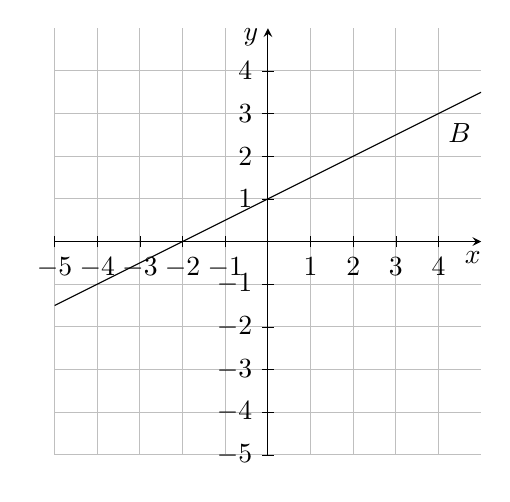
\begin{tikzpicture}[domain=-5:5,smooth]
  \begin{axis}[
      width=7cm,height=7cm,
      axis lines=middle,
      domain=-5:5,
      smooth,
      no markers,
      grid,
      xmin=-5,xmax=5,
      tick style=black,
      xtick={-5,-4,...,4},
      xlabel=$x$,
      xlabel style={below, anchor=north east,inner xsep=0pt},
      restrict y to domain=-9:9,
      ymin=-5,ymax=5,
      ytick={-5,-4,...,4},ylabel=$y$,
      ylabel style={above,anchor=north east,inner ysep=0pt},
      samples=100,
    ]
    \addplot[color=black]{0.5*x+1}node[pos=0.9,below right]{$B$};
  \end{axis}
\end{tikzpicture}}
\scalebox{0.8}{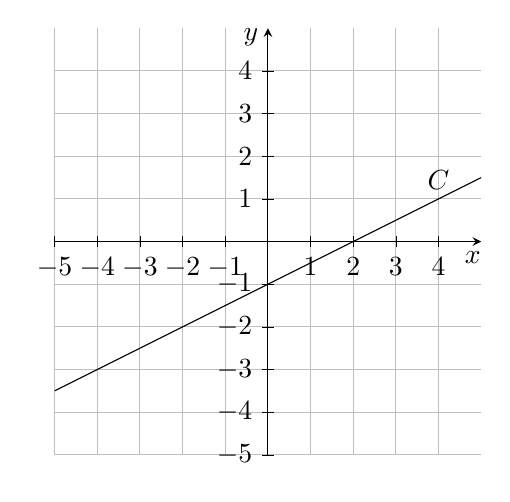
\begin{tikzpicture}[domain=-5:5,smooth]
  \begin{axis}[
      width=7cm,height=7cm,
      axis lines=middle,
      domain=-5:5,
      smooth,
      no markers,
      grid,
      xmin=-5,xmax=5,
      tick style=black,
      xtick={-5,-4,...,4},
      xlabel=$x$,
      xlabel style={below, anchor=north east,inner xsep=0pt},
      restrict y to domain=-9:9,
      ymin=-5,ymax=5,
      ytick={-5,-4,...,4},ylabel=$y$,
      ylabel style={above,anchor=north east,inner ysep=0pt},
      samples=100,
    ]
    \addplot[color=black]{0.5*x-1}node[pos=0.9,above]{$C$};
  \end{axis}
\end{tikzpicture}}

\scalebox{0.8}{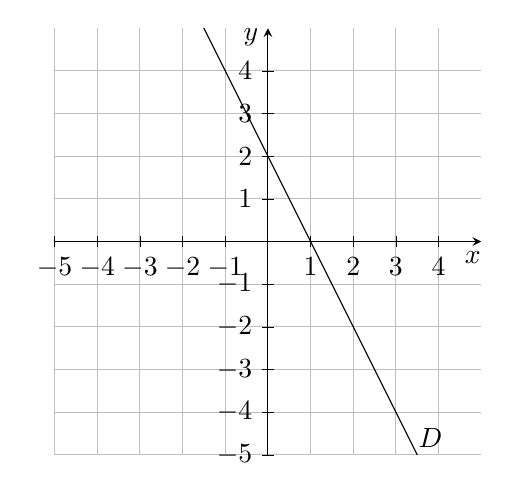
\begin{tikzpicture}[domain=-5:5,smooth]
  \begin{axis}[
      width=7cm,height=7cm,
      axis lines=middle,
      domain=-5:5,
      smooth,
      no markers,
      grid,
      xmin=-5,xmax=5,
      tick style=black,
      xtick={-5,-4,...,4},
      xlabel=$x$,
      xlabel style={below, anchor=north east,inner xsep=0pt},
      restrict y to domain=-9:9,
      ymin=-5,ymax=5,
      ytick={-5,-4,...,4},ylabel=$y$,
      ylabel style={above,anchor=north east,inner ysep=0pt},
      samples=100,
    ]
    \addplot[color=black]{-2*x+2}node[pos=0.8,right]{$D$};
  \end{axis}
\end{tikzpicture}}
\scalebox{0.8}{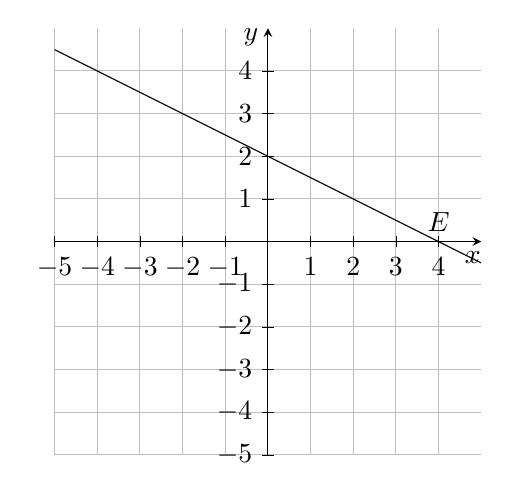
\begin{tikzpicture}[domain=-5:5,smooth]
  \begin{axis}[
      width=7cm,height=7cm,
      axis lines=middle,
      domain=-5:5,
      smooth,
      no markers,
      grid,
      xmin=-5,xmax=5,
      tick style=black,
      xtick={-5,-4,...,4},
      xlabel=$x$,
      xlabel style={below, anchor=north east,inner xsep=0pt},
      restrict y to domain=-9:9,
      ymin=-5,ymax=5,
      ytick={-5,-4,...,4},ylabel=$y$,
      ylabel style={above,anchor=north east,inner ysep=0pt},
      samples=100,
    ]
    \addplot[color=black]{-0.5*x+2}node[pos=0.9,above]{$E$};
  \end{axis}
\end{tikzpicture}}
\begin{table}[h!]
\renewcommand{\arraystretch}{2}
\begin{tabular}{|M{3.2cm}|M{3.2cm}|M{3.2cm}|M{3.2cm}|M{3.2cm}|}
\hline
$f_1=0,5x+1$ & $f_2(x)=0,5x-1$ & $f_3(x)=-0,5x+2$ & $f_4(x)=-2x+2$ & $f_5(x)=2x-1$ \\ \hline
 & & & & \\ \hline
\end{tabular}
\end{table}

\droptotalpoints

\question[3]

Zeichne ein Steigungsdreieck in das folgende Diagramm. Bestimme die Steigung $m$ und den Achsenabschnitt $b$. Notiere anschließend die Funktionsgleichung.

\begin{minipage}{0.5\textwidth}
\pgfplotsset{
  compat=1.12,
  axis lines=middle
}
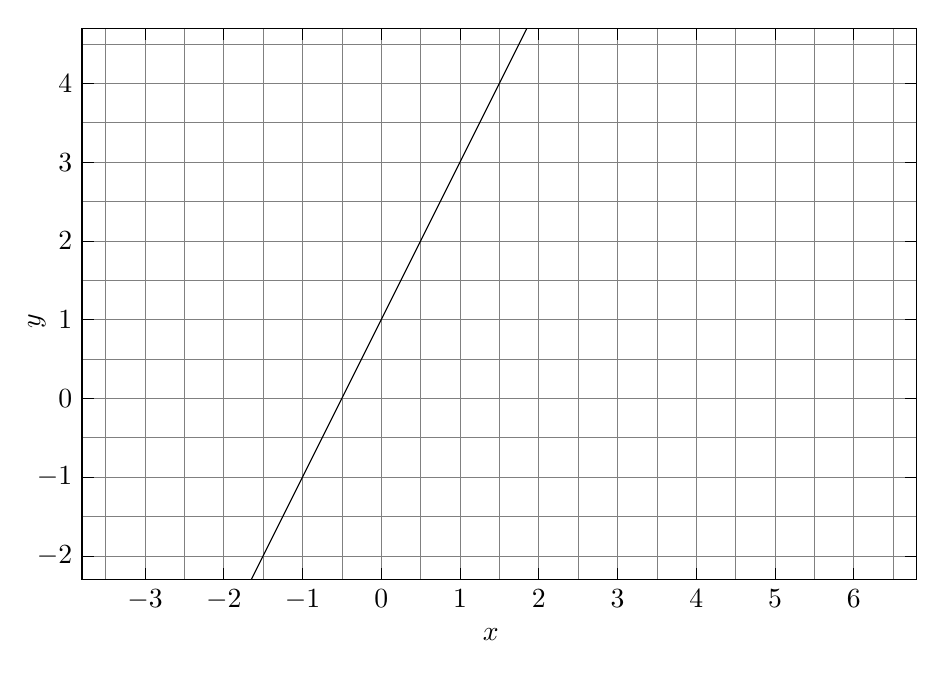
\begin{tikzpicture}
  \begin{axis}[
    xlabel=$x$,
    xlabel style={below, anchor=north east,inner xsep=0pt},
    ylabel=$y$,
    ylabel style={above,anchor=north east,inner ysep=0pt},
    xmin=-3.8,xmax=6.8,
    ymin=-2.3,ymax=4.7,
    x=1cm,
    y=1cm,
    tick style=black,
    set layers
    ]
    \pgfplotsinvokeforeach {-10,-9.5,...,10}{
      \pgfonlayer{axis grid}
        \begin{scope}
          \clip(current axis.south west)rectangle(current axis.north east);
          \draw[help lines](#1,0|-current axis.south)--(#1,0|-current axis.north);
          \draw[help lines](0,#1-|current axis.west)--(0,#1-|current axis.east);
        \end{scope}
      \endpgfonlayer
    }
    \addplot[color=black]{2*x+1}node[pos=1, below right]{$f$};
  \end{axis}
\end{tikzpicture}
\end{minipage}\begin{minipage}{0.5\textwidth}
\begin{align*}
    m=&\loeslin\\[0.5cm]
    b=&\loeslin\\[0.5cm]
    y=&\loeslinl
\end{align*}
\end{minipage}

\droptotalpoints

\question Bei seinem Vertrag mit SuperPhone zahlt Herr Schmidt eine Handygrundgebühr von 10\euro. Für jede Minute, der Herr Schmidt telefoniert, zahlt er $0,10$\euro.
\begin{parts}
\part[1] Wie viel muss Herr Schmidt bezahlen, wenn er in einem Monat 45 Minuten telefoniert? \droppoints
\gridsolution{8+45*0,1 = 12,5[€]}{2cm}
\part[2] Wie viel muss Herr Schmidt bezahlen, wenn er 1,5h telefoniert? \droppoints
\gridsolution{8+90*0,1 = 17[€]}{2cm}
\part[2] Gib eine passende Funktionsgleichung an, mit der der Rechnungsbetrag bestimmt werden kann. \droppoints
\gridsolution{8+45*0,1 = 12,5[€]}{2cm}
\part[2] Zeichne den Graphen in das Koordinatensystem \droppoints

\pgfplotsset{
  compat=1.12,
  axis lines=middle
}
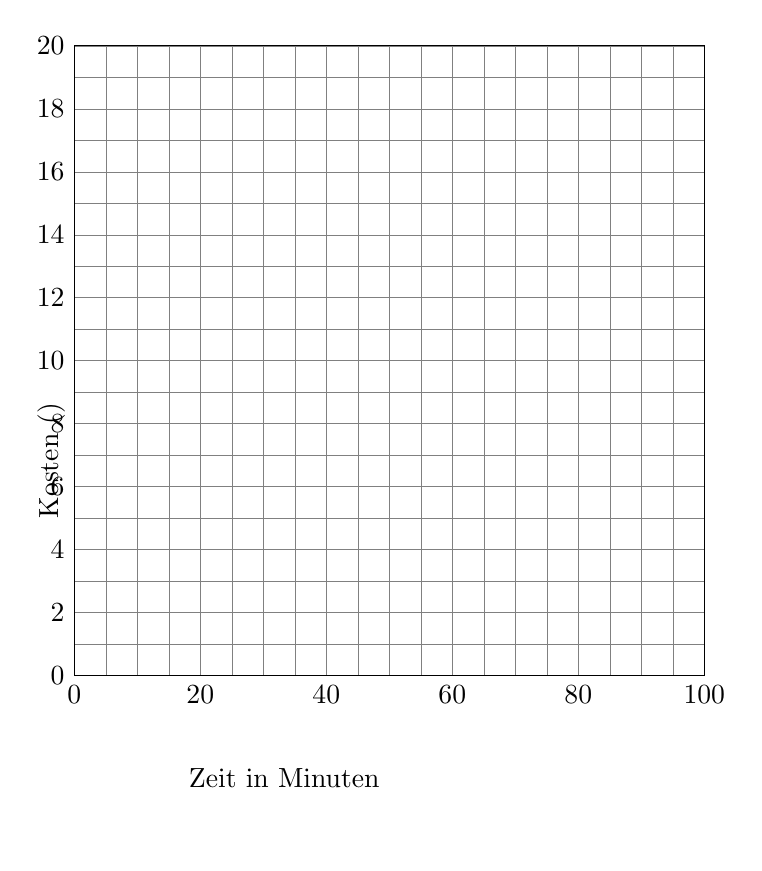
\begin{tikzpicture}[scale=1]
  \begin{axis}[
    xlabel=Zeit in Minuten,
    xlabel style={below, anchor=north east,inner ysep=20pt},
    ylabel=Kosten (\euro),
    ylabel style={above,anchor=north east,inner xsep=15pt},
    xmin=0,xmax=100,
    ymin=0,ymax=20,
    x=0.08cm,
    y=0.4cm,
    set layers
    ]
    \pgfplotsinvokeforeach {-100,-95,...,100}{
      \pgfonlayer{axis grid}
        \begin{scope}
          \clip(current axis.south west)rectangle(current axis.north east);
          \draw[help lines](#1,0|-current axis.south)--(#1,0|-current axis.north);
        \end{scope}
      \endpgfonlayer
    }
    \pgfplotsinvokeforeach {-100,-99,...,100}{
      \pgfonlayer{axis grid}
        \begin{scope}
          \clip(current axis.south west)rectangle(current axis.north east);
          \draw[help lines](0,#1-|current axis.west)--(0,#1-|current axis.east);
        \end{scope}
      \endpgfonlayer
    }
  \end{axis}
\end{tikzpicture}
\end{parts}

\droptotalpoints
\newpage
\question[3]
Drei Geraden treffen sich im Punkt $P(2|1)$

Sie führen eine kleine Unterhaltung:

\glqq Meine Steigung ist zwei\grqq , erklärt Gerade $f$.

\glqq Zu mir gehört auch der Punkt $Q(4|-1)$\grqq , sagt Gerade g.

\glqq Meine Gleichung habe ich leider vergessen. Ich weiß aber noch, dass ich eine proportionale Funktion bin\grqq, sagt Gerade $h$.

Zeichne die drei Geraden in das untenstehende Koordinatensystem.

\pgfplotsset{
  compat=1.12,
  axis lines=middle
}
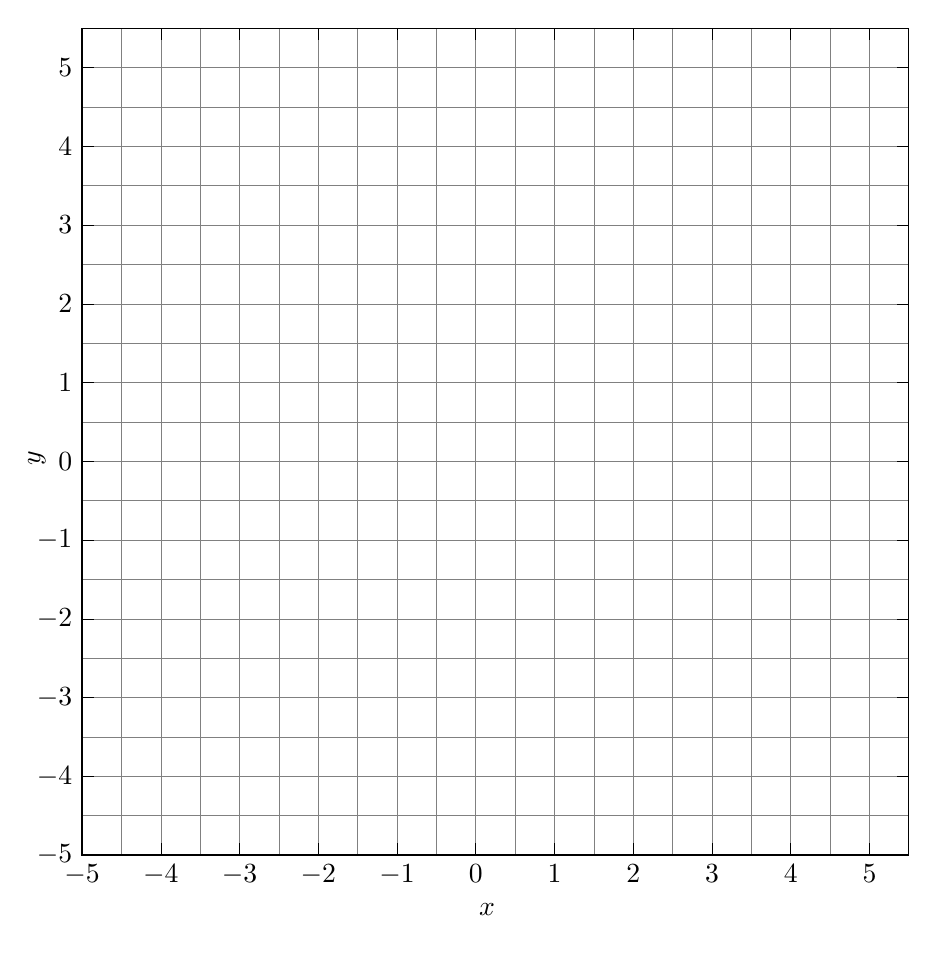
\begin{tikzpicture}
  \begin{axis}[
    xlabel=$x$,
    xlabel style={below, anchor=north east,inner xsep=0pt},
    ylabel=$y$,
    ylabel style={above,anchor=north east,inner ysep=0pt},
    xmin=-5,xmax=5.5,
    ymin=-5,ymax=5.5,
    tick style=black,
    x=1cm,
    y=1cm,
    set layers
    ]
    \pgfplotsinvokeforeach {-10,-9.5,...,10}{
      \pgfonlayer{axis grid}
        \begin{scope}
          \clip(current axis.south west)rectangle(current axis.north east);
          \draw[help lines](#1,0|-current axis.south)--(#1,0|-current axis.north);
          \draw[help lines](0,#1-|current axis.west)--(0,#1-|current axis.east);
        \end{scope}
      \endpgfonlayer
    }
  \end{axis}
\end{tikzpicture}

\droptotalpoints

\question
\begin{parts}
\part[2] Die Punkte $A$ und $B$ liegen auf der Normalparabel. Bestimme die fehlende $y$-Koordinaten. \droppoints

$A(2,5|\loeslin) \quad B(-1,5|\loeslin)$
\part[1] Der Punkt $C$ liegt auf der an der $x$-Achse gespiegelten Normalparabel. Bestimme die fehlende $y$-Koordinate. \droppoints

$C(-1,5|\loeslin)$
\end{parts}
\droptotalpoints

\question[3]
Gegeben ist die Funktion $f$ mit $f(x)=-2,3x^2 - 1$. Kreuze an, welche der Punkte auf dem Graphen von $f$ liegen.

\begin{oneparcheckboxes}
\choice $P(0|-1)$
\choice $P(3|21,7)$
\choice $P(-2|-10,2)$
\end{oneparcheckboxes}

\droptotalpoints

\question[2] Kreuze die wahren Aussagen an.

\begin{checkboxes}
\choice $f_1$ gegeben durch $f_1(x)=5x^2$ ist enger als die Normalparabel.
\choice $f_2$ gegeben durch $f_2(x)=-2x^2$ ist nach oben geöffnet.
\choice $f_3$ gegeben durch $f_3(x)=0,1x^2$ ist enger als die Normalparabel.
\choice $f_4$ gegeben durch $f_4(x)=-\frac{3}{4}x^2$ nach unten geöffnet.
\end{checkboxes}

\droptotalpoints

\question[5]

Ordne den Funktionsgraphen die korrekte Funktionsgleichung zu. 
\begin{center}
\pgfplotsset{
  compat=1.12,
  axis lines=middle
}
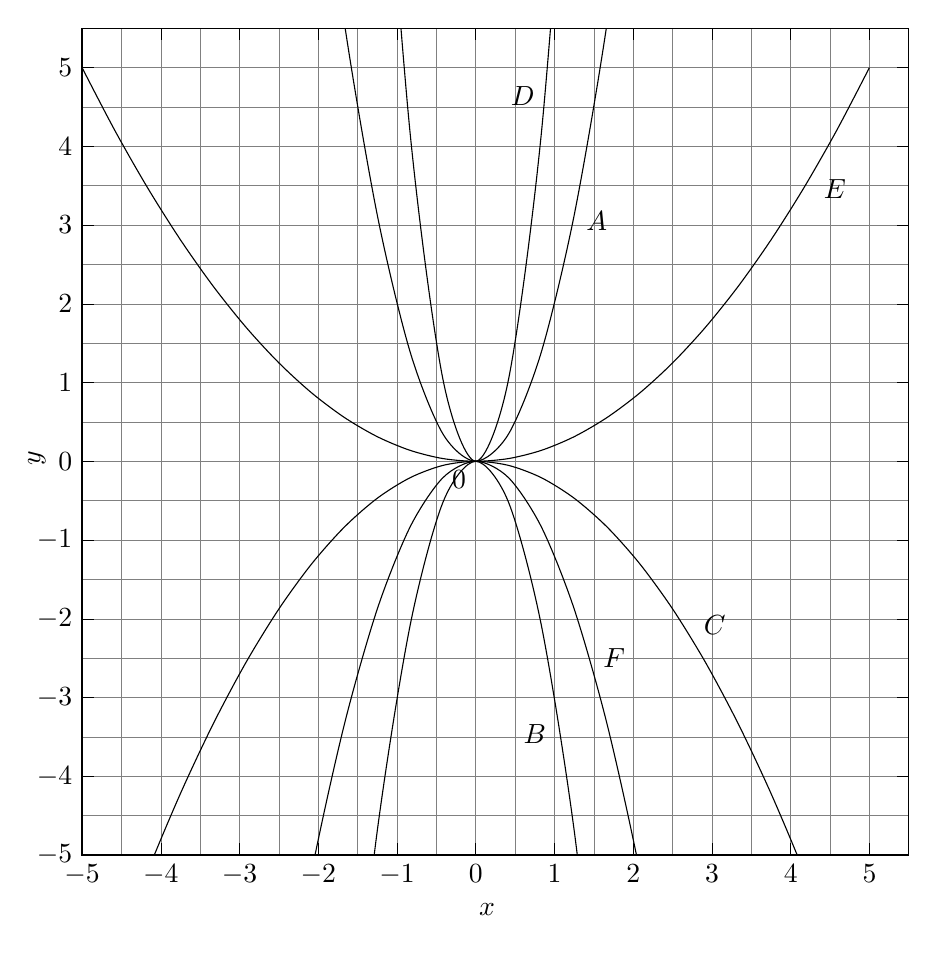
\begin{tikzpicture}
  \begin{axis}[
    xlabel=$x$,
    xlabel style={below, anchor=north east,inner xsep=0pt},
    ylabel=$y$,
    ylabel style={above,anchor=north east,inner ysep=0pt},
    xmin=-5,xmax=5.5,
    ymin=-5,ymax=5.5,
    x=1cm,
    y=1cm,
    tick style=black,
    restrict y to domain=-10:10,
    set layers
    ]
    \pgfplotsinvokeforeach {-10,-9.5,...,10}{
      \pgfonlayer{axis grid}
        \begin{scope}
          \clip(current axis.south west)rectangle(current axis.north east);
          \draw[help lines](#1,0|-current axis.south)--(#1,0|-current axis.north);
          \draw[help lines](0,#1-|current axis.west)--(0,#1-|current axis.east);
        \end{scope}
      \endpgfonlayer
    }
    \node [anchor=north east] at (0, 0) {$0$};
    \addplot[color=black,smooth]{2*x*x}node[pos=0.7,below right]{$A$};
    \addplot[color=black,smooth]{-3*x*x}node[pos=0.7, below left]{$B$};
    \addplot[color=black,smooth]{-0.3*x*x}node[pos=0.7, above right ]{$C$};
    \addplot[color=black,smooth]{6*x*x}node[pos=0.75, left]{$D$};
    \addplot[color=black,smooth]{0.2*x*x}node[pos=0.9, below right]{$E$};
    \addplot[color=black,smooth]{-1.2*x*x}node[pos=0.7, above right]{$F$};
  \end{axis}
\end{tikzpicture}
\end{center}
\begin{align*}
f_1(x)&=2x^2  &  f_2(x) &=6x^2    &  f_3(x) &=0,2x^2 \\
f_4(x)&=-3x^2 &  f_5(x) &=-0,3x^2    &  f_6(x) &=-1,2x^2 
\end{align*}

\begin{table}[h!]
\renewcommand{\arraystretch}{2}
\begin{tabular}{|M{2.2cm}|M{2.2cm}|M{2.2cm}|M{2.2cm}|M{2.2cm}|M{2.2cm}|}
\hline
$A$ & $B$ & $C$ & $D$ & $E$ & $F$ \\ \hline
 & & & & & \\ \hline
\end{tabular}
\end{table}

\droptotalpoints

\newpage

\question Gib die Koordinaten der Scheitelpunkte an.

\begin{parts}
    \part[1] $f(x)=(x-3)^2-4 \qquad S(\loeslin | \loeslin)$ \droppoints
    \part[1] $f(x)=(x+2)^2-1 \qquad S(\loeslin | \loeslin)$ \droppoints
    \part[1] $f(x)=(x-1)^2 \qquad S(\loeslin | \loeslin)$ \droppoints
\end{parts}

\droptotalpoints

\question
Die Abbildung zeigt die Parabel $p$ mit der Funktionsgleichung $p(x)=x^2+6x+7$.

\pgfplotsset{
  compat=1.18,
  axis lines=middle
}
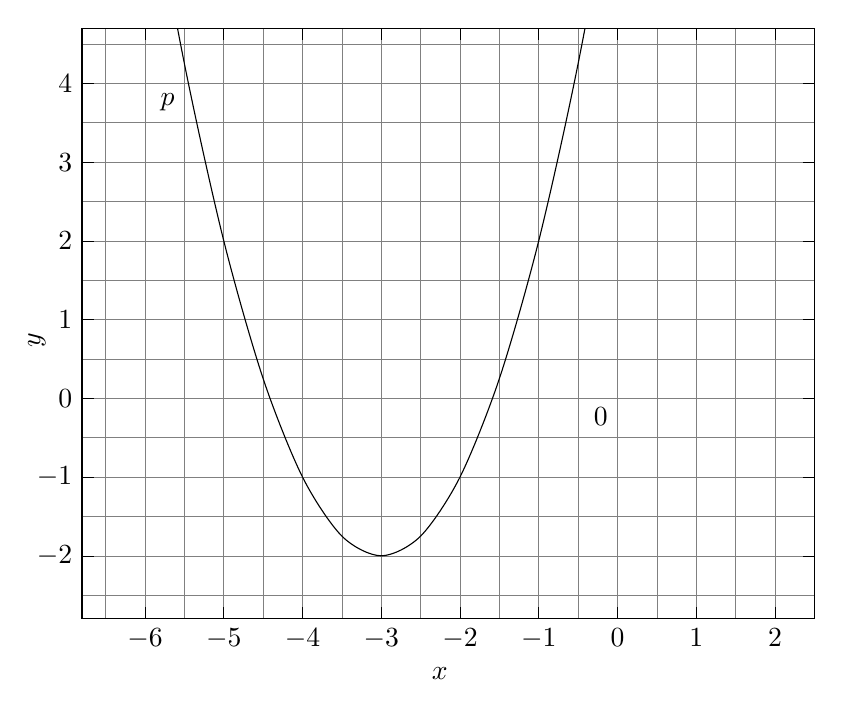
\begin{tikzpicture}[domain=-7:5,smooth]
  \begin{axis}[
    xlabel=$x$,
    xlabel style={below, anchor=north east,inner xsep=0pt},
    ylabel=$y$,
    ylabel style={above,anchor=north east,inner ysep=0pt},
    xmin=-6.8,xmax=2.5,
    ymin=-2.8,ymax=4.7,
    x=1cm,
    y=1cm,
    tick style=black,
    set layers
    ]
    \pgfplotsinvokeforeach {-10,-9.5,...,10}{
      \pgfonlayer{axis grid}
        \begin{scope}
          \clip(current axis.south west)rectangle(current axis.north east);
          \draw[help lines](#1,0|-current axis.south)--(#1,0|-current axis.north);
          \draw[help lines](0,#1-|current axis.west)--(0,#1-|current axis.east);
        \end{scope}
      \endpgfonlayer
    }
    \node [anchor=north east] at (0, 0) {$0$};
    \addplot[color=black,smooth]{x*x+6*x+7};
    \node [anchor=north east] at (-5.5, 4) {$p$};
  \end{axis}
\end{tikzpicture}
\begin{parts}
    \part[1] Markiere den Scheitelpunkt in dem Diagramm. \droppoints
    \part[2] Gib die Funktionsgleichung für die Parabel $p$ in Scheitelpunktform an. \droppoints
\vspace{0.5cm}

\begin{center}
    $p(x)=\loeslinl$
\end{center}
\end{parts}
\droptotalpoints
\nomorequestions
\end{questions}
\end{document}